%%%%%%%%%%%%%%%%%%%%%%%%%%%%%%%%%%%%%%%%%
% Beamer Presentation
% LaTeX Template
% Version 1.0 (10/11/12)
%
% This template has been downloaded from:
% http://www.LaTeXTemplates.com
%
% License:
% CC BY-NC-SA 3.0 (http://creativecommons.org/licenses/by-nc-sa/3.0/)
%
%%%%%%%%%%%%%%%%%%%%%%%%%%%%%%%%%%%%%%%%%

%----------------------------------------------------------------------------------------
%	PACKAGES AND THEMES
%----------------------------------------------------------------------------------------

\documentclass{beamer}

\mode<presentation> {

% The Beamer class comes with a number of default slide themes
% which change the colors and layouts of slides. Below this is a list
% of all the themes, uncomment each in turn to see what they look like.

%\usetheme{default}
%\usetheme{AnnArbor}
%\usetheme{Antibes}
%\usetheme{Bergen}
%\usetheme{Berkeley}
%\usetheme{Berlin}
%\usetheme{Boadilla}
%\usetheme{CambridgeUS}
%\usetheme{Copenhagen}
%\usetheme{Darmstadt}
%\usetheme{Dresden}
%\usetheme{Frankfurt}
%\usetheme{Goettingen}
%\usetheme{Hannover}
%\usetheme{Ilmenau}
%\usetheme{JuanLesPins}
%\usetheme{Luebeck}
\usetheme{Madrid}
%\usetheme{Malmoe}
%\usetheme{Marburg}
%\usetheme{Montpellier}
%\usetheme{PaloAlto}
%\usetheme{Pittsburgh}
%\usetheme{Rochester}
%\usetheme{Singapore}
%\usetheme{Szeged}
%\usetheme{Warsaw}

% As well as themes, the Beamer class has a number of color themes
% for any slide theme. Uncomment each of these in turn to see how it
% changes the colors of your current slide theme.

%\usecolortheme{albatross}
%\usecolortheme{beaver}
%\usecolortheme{beetle}
%\usecolortheme{crane}
%\usecolortheme{dolphin}
%\usecolortheme{dove}
%\usecolortheme{fly}
%\usecolortheme{lily}
%\usecolortheme{orchid}
%\usecolortheme{rose}
%\usecolortheme{seagull}
%\usecolortheme{seahorse}
%\usecolortheme{whale}
%\usecolortheme{wolverine}

%\setbeamertemplate{footline} % To remove the footer line in all slides uncomment this line
%\setbeamertemplate{footline}[page number] % To replace the footer line in all slides with a simple slide count uncomment this line

%\setbeamertemplate{navigation symbols}{} % To remove the navigation symbols from the bottom of all slides uncomment this line
}

\usepackage{graphicx} % Allows including images
\usepackage{booktabs} % Allows the use of \toprule, \midrule and \bottomrule in tables

%----------------------------------------------------------------------------------------
%	TITLE PAGE
%----------------------------------------------------------------------------------------

\title[FiQuant Market Simulator]{Market Microstructure Simulator: Strategy Definition Language} % The short title appears at the bottom of every slide, the full title is only on the title page

\author{Anton Kolotaev} % Your name
\institute[ECP] % Your institution as it will appear on the bottom of every slide, may be shorthand to save space
{
Chair of Quantitative Finance, \'{E}cole Centrale Paris \\ % Your institution for the title page
\medskip
\textit{anton.kolotaev@gmail.com} % Your email address
}
\date{\today} % Date, can be changed to a custom date

\begin{document}

\begin{frame}
\titlepage % Print the title page as the first slide
\end{frame}

\begin{frame}
\frametitle{Overview} % Table of contents slide, comment this block out to remove it
\tableofcontents % Throughout your presentation, if you choose to use \section{} and \subsection{} commands, these will automatically be printed on this slide as an overview of your presentation
\end{frame}

%----------------------------------------------------------------------------------------
%	PRESENTATION SLIDES
%----------------------------------------------------------------------------------------

%------------------------------------------------
\section{Introduction}
\subsection{History}
%------------------------------------------------
\begin{frame}
\frametitle{Evolution of the simulator I}
\begin{enumerate}
  \item Initial C++ version was developed in 2009-2011 by Riadh Zaatour. In this version a user implements strategy logic in C++. Though this version was quite easy to learn and understand, it had problems with flexibility and scalability.
  \item In order to improve its extensibility and performance the simulator was rewritten using C++ template metaprogramming techniques by Anton Kolotaev in 2012. Python bindings to it were implemented using Boost.Python. Unfortunately the price for providing high extensibility with no overhead was quite high: in order to use it a proficiency in C++ template metaprogramming was required.
\end{enumerate}
\end{frame}
%------------------------------------------------
\begin{frame}
\frametitle{Evolution of the simulator II}
\begin{enumerate}
  \item In order to make the simulator easy to start work with, a Python version with a Web interface was developed in 2013. Karol Podkanski implemented number of trading strategies and indicators during his internship at summer 2013. Though this version gave a lot of insights on how a good modular design for market simulation software should be implemented, it showed that a lot of syntax noise appears in strategy description and the development becomes very error-prone because of the dynamic typing nature of Python.
  \item In October 2013 a decision to introduce a strategy definition language and a compiler for it was taken.
\end{enumerate}
\end{frame}
%------------------------------------------------
\subsection{Design}
\begin{frame}
\frametitle{Design goals}
\begin{enumerate}
  \item \textbf{\textit{Flexibility}}. A simulation library must have a very modular design in order to provide a high level of flexibility to the user. This requirement comes from the original purpose of a simulation as a test bed for experiments with different models and parameters.
  \item \textbf{\textit{Used-friendliness}}. Since a typical simulation model is composed of many hundreds and thousands blocks, it is very important to provide a simple way for user to tell how a behaviour wanted differs from the default one. Simulator API should be friendly to modern IDEs
  \item \textbf{\textit{Performance}}. A user should be allowed to choose between small start-up time and high simulation speed.
\end{enumerate}
\end{frame}
%------------------------------------------------
\begin{frame}
\frametitle{Modular Design}
Representing a simulation model as a \textbf{network} of modules communicating by \textbf{messages} is a widely accepted practice for DES systems (e.g. Omnet++ or ns-2 to simulate telecommunication networks).

Module may have \textbf{parameters} that are used to adjust their behaviour. Modules are organized into \textbf{hierarchy} in order to facilitate construction of large-scale simulation.

We will distinguish two sorts of modules:
\begin{enumerate}
\item \textbf{\textit{Simple modules}} provide functionality which is considered elementary (and there is no reason to reuse part of it to implement other modules).

\item \textbf{\textit{Compound modules}} combine together other modules in some way and define their parameters based on its own parameters. Compound module behaviour is just a composition of its constituting modules behaviours.
\end{enumerate}
\end{frame}
%------------------------------------------------

\begin{frame}
\frametitle{Modular design sample: Crossing Averages Strategy}
\begin{figure}[htbp]
\centering
\includegraphics[width=1\linewidth]{graph.png}
\end{figure}
\end{frame}
%------------------------------------------------
\subsection{DSL}
\begin{frame}
\frametitle{Motivation for an external DSL}
\begin{enumerate}
  \item \textbf{\textit{Syntax}}. We may design an external DSL so its syntax describes very well domain specific abstractions.
  \item \textbf{\textit{Error checking}}. A DSL compiler can detect incorrect parameter values as soon as possible thus shortening simulation development cycle and facilitating refactorings.
  \item \textbf{\textit{Multiple target languages}}. A DSL can be compiled into different languages: e.g. into Python to provide fast start-up and into C++ to have highly optimized fast simulations. A new target language introduced, only simple modules need to be re-written into it; compound modules will be ported automatically.
  \item \textbf{\textit{IDE support}}. Modern IDEs like Eclipse, Intellij IDEA allow writing plug-ins that would provide smart syntax highlighting, auto-completion and check errors on-the-fly for user-defined DSLs.
  \item \textbf{\textit{High-level optimizations}} are easier to implement. 
\end{enumerate}
\end{frame}
%------------------------------------------------
\begin{frame}
\frametitle{Scala as a language to implement the DSL compiler}
\begin{enumerate}
  \item As a ML-family member, very suitable for sophisticated symbol processing tasks like compilation: an internal DSL to parse texts, algebraic data types, pattern matching, a powerful collections library, mixin inheritance via traits.
  \item Good balance between functional and imperative programming features -- easier to find software engineers
  \item The most mainstream of functional programming languages that results in wide community, excellent library and tool support, mature IDEs.
  \item Very portable since runs on JVM.
  \item Statically typed
  \item Right choice to develop a Web server.
\end{enumerate}
\end{frame}
%------------------------------------------------
\section{Strategy Definition Language}
\subsection{Functions}
\begin{frame}
\frametitle{Functions}
Conceptually, a "function" declaration defines a term with a constructor provided (like case classes in Scala). 

Types for input arguments are inferred automatically from their initializers and for the "return" value - from the function body.

Functions represent compound modules of a simulation model.

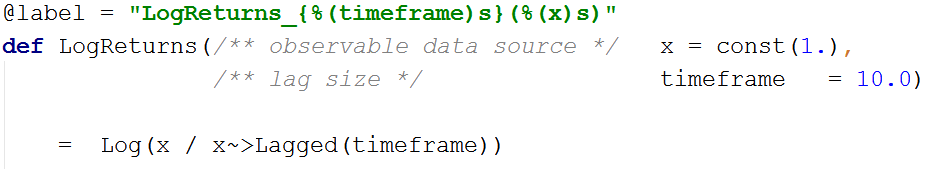
\includegraphics[width=1\linewidth]{logreturns.png}

All methods can be considered as extension methods of their first argument. 

\texttt{x$\sim$>Lagged(dt)} is equivalent to \texttt{.observable.Lagged(x, dt)}.
\end{frame}
%------------------------------------------------
\begin{frame}
\frametitle{Intrinsic Functions}
Intrinsic functions import simple modules from a target language into the DSL. 
"Return" types for intrinsic functions must be specified explicitly.
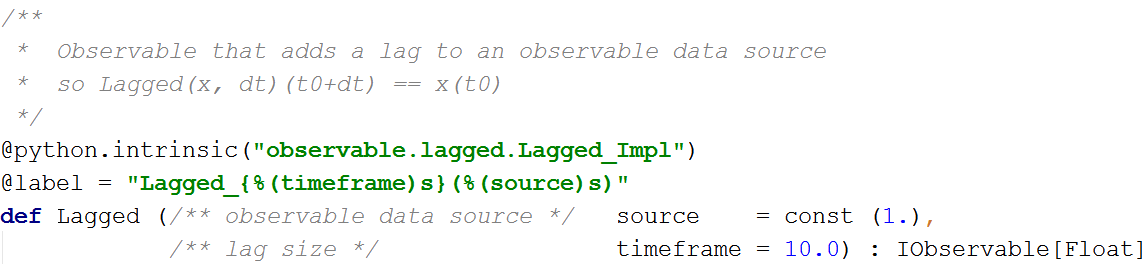
\includegraphics[width=1\linewidth]{lagged.png}
\end{frame}
%------------------------------------------------
\subsection{Types}
\begin{frame}
\frametitle{Type System I}
Types correspond to interfaces without methods from mainstream languages. They are used for error checking and for function overloading.
\begin{enumerate}
  \item Simple types may derive from other types or be aliases
  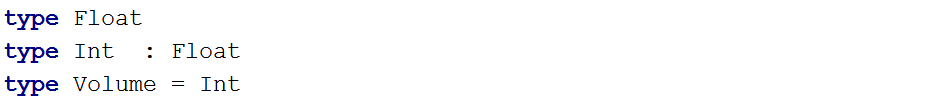
\includegraphics[width=1\linewidth]{intfloat.png}
  \item Tuple and function types
  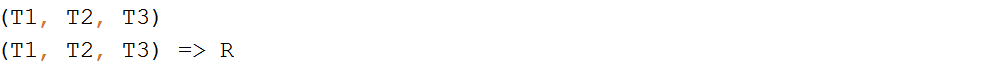
\includegraphics[width=1\linewidth]{tuplefunction.png}
  \item Top (\texttt{Any}) and bottom (\texttt{Nothing}) types.
  \item Lists (\texttt{List[T]})
\end{enumerate}
\end{frame}
%------------------------------------------------
\begin{frame}
\frametitle{Type System II}
Types may be generic. 

Functions are contravariant in the input type and covariant in the output type: \texttt{CanCast(D,B)} $\wedge$ \texttt{CanCast(R,T)} $\Rightarrow$ \texttt{CanCast(B=>R,D=>T)}.

All other types are covariant.

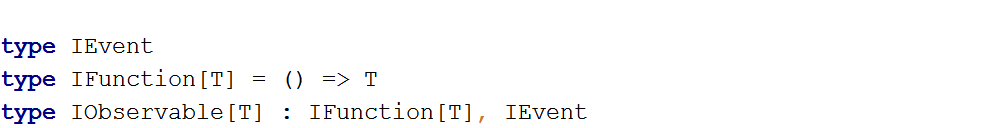
\includegraphics[width=1\linewidth]{iobservable.png}

\end{frame}
%------------------------------------------------
\subsection{Classes}
\begin{frame}
\frametitle{Classes I}
Classes are syntax sugar for a type declaration, constructor function and member accessors

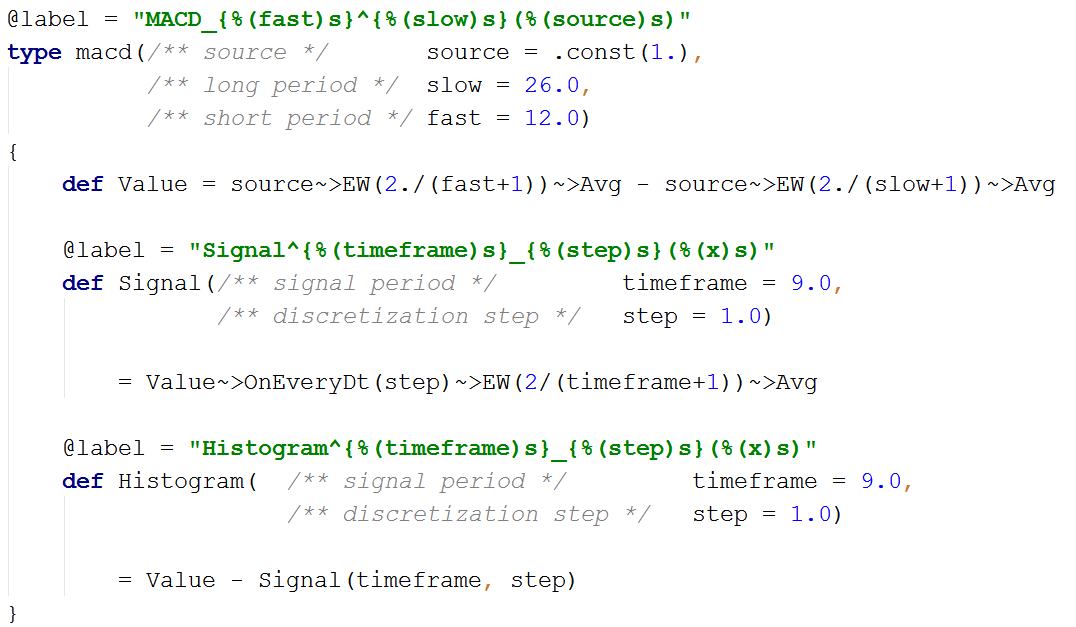
\includegraphics[width=1\linewidth]{macd.png}

\end{frame}
%------------------------------------------------
\begin{frame}
\frametitle{Classes II}
Previous definition is de-sugared at typing stage into

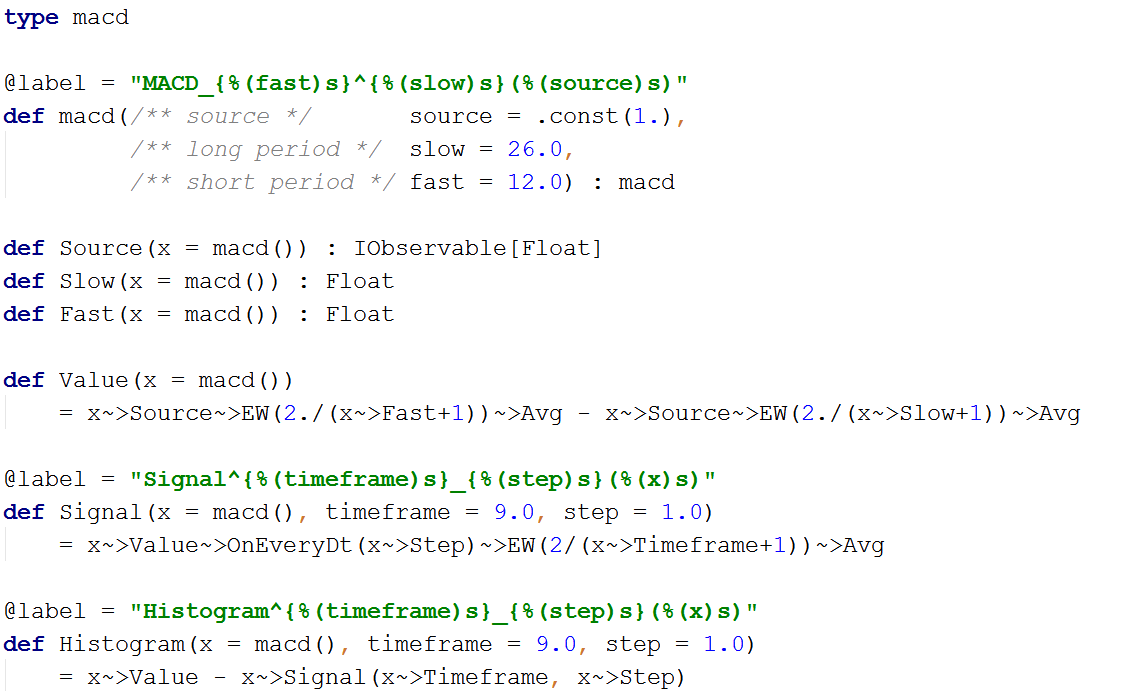
\includegraphics[width=1\linewidth]{macd_desugared.png}
\end{frame}
%------------------------------------------------
\begin{frame}
\frametitle{Class Inheritance}
Classes derive fields and methods from base classes.

Methods are treated as "virtual" to stimulate code re-use

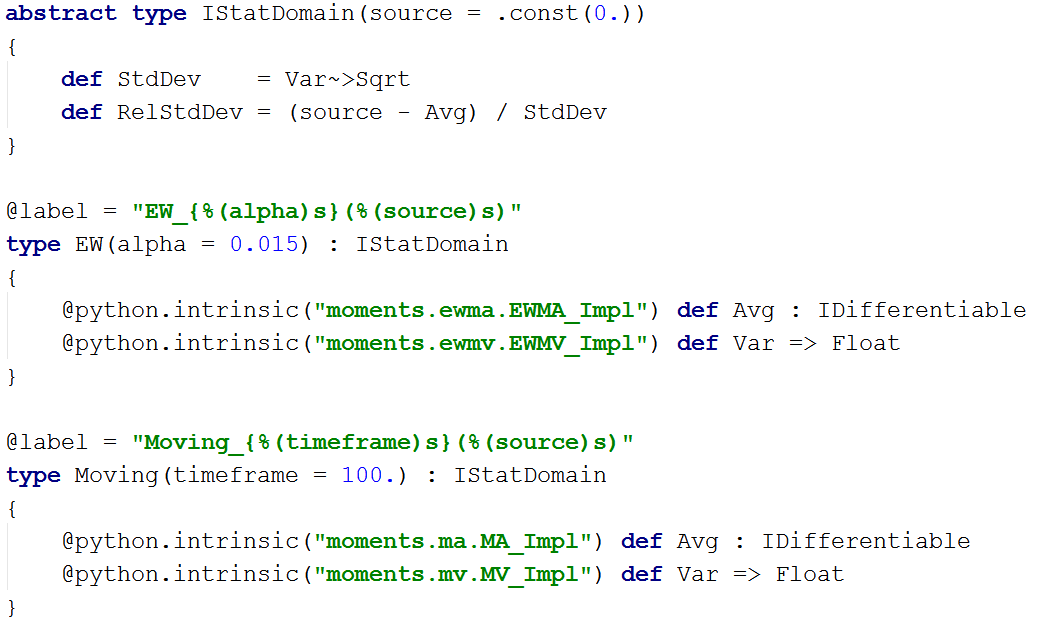
\includegraphics[width=1\linewidth]{moments.png}
\end{frame}
%------------------------------------------------
\subsection{Packages}
\begin{frame}
\frametitle{Packages and Attributes}
Packages are used to group functions and types. They can be nested. Attributes are inherited from enclosing package. Anonymous packages are used to assign same attributes to a group of functions without introducing a new name scope.

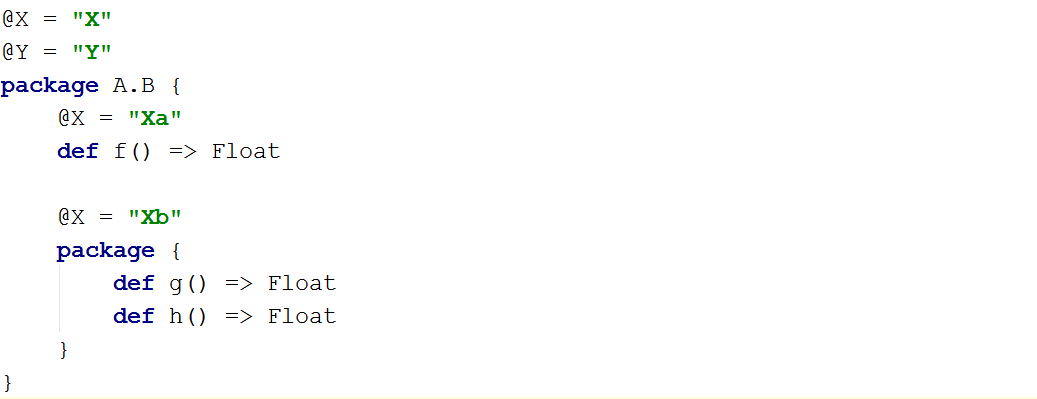
\includegraphics[width=1\linewidth]{packages.png}

In this sample \texttt{.A.B.f} will have attributes \texttt{X == "Xa", Y == "Y"} and \texttt{.A.B.g} and \texttt{.A.B.h} will have attributes \texttt{X == "Xb", Y == "Y"}

\end{frame}
%------------------------------------------------
\begin{frame}
\frametitle{Example: Relative Strength Index}
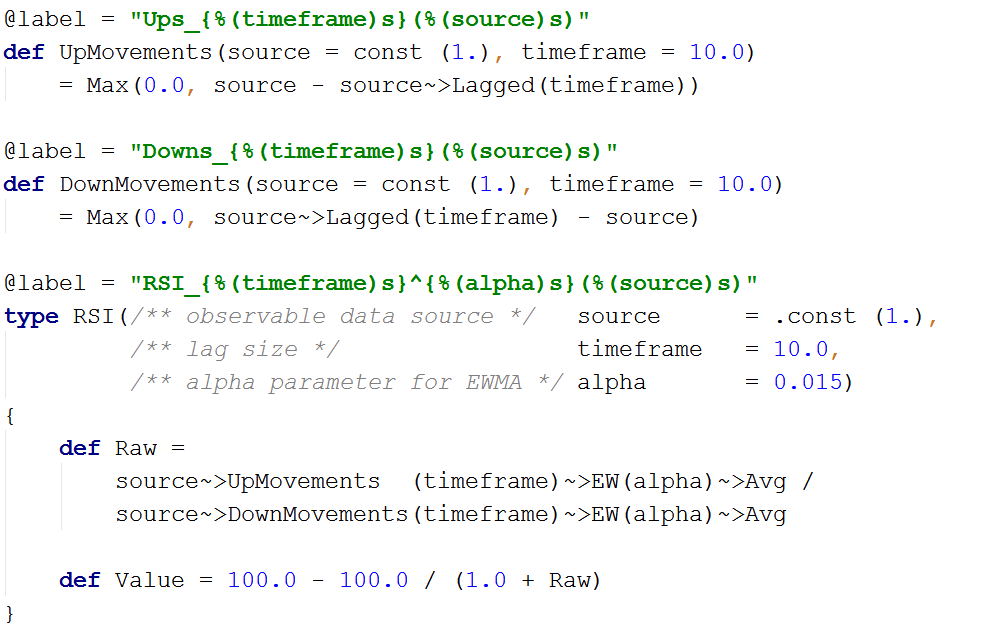
\includegraphics[width=1\linewidth]{rsi.png}
\end{frame}
%------------------------------------------------
\section{Strategies}
\subsection{Position strategies}
\begin{frame}
\frametitle{Relative Strength Index Strategy}
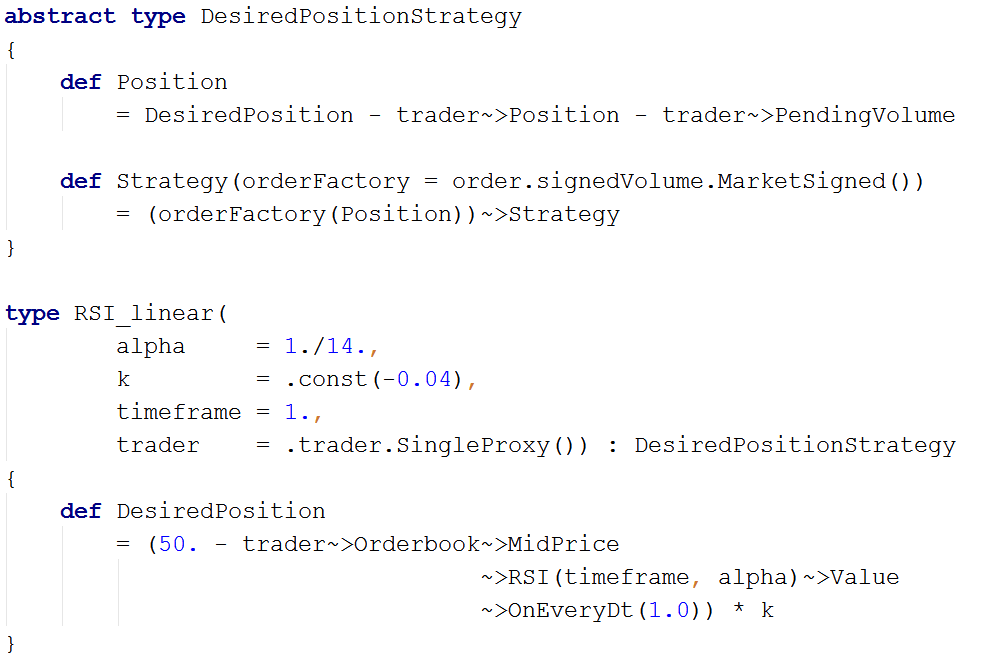
\includegraphics[width=1\linewidth]{rsi_strategy.png}
\end{frame}
%------------------------------------------------
\begin{frame}
\frametitle{Bollinger Bands Strategy}
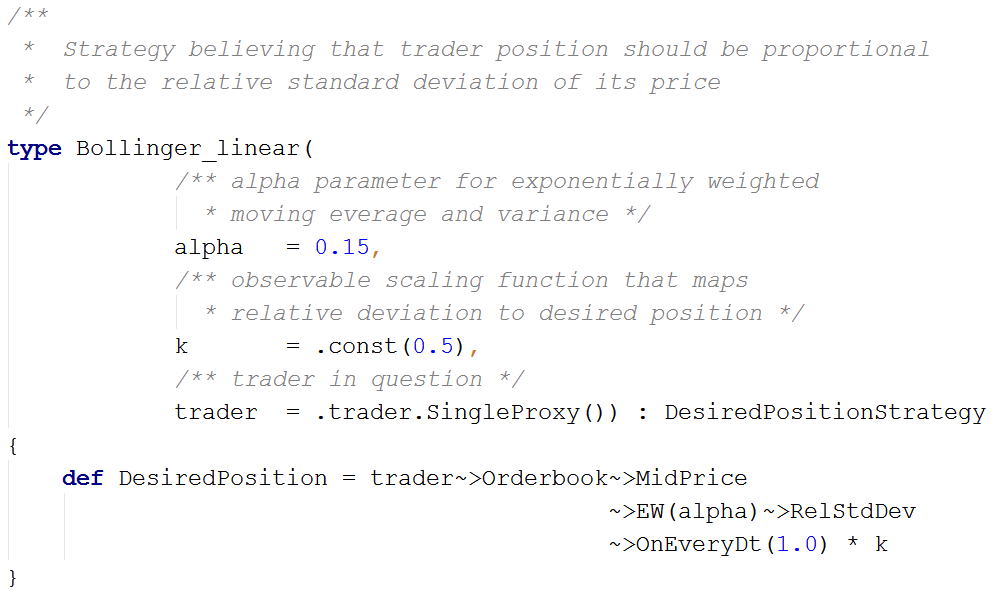
\includegraphics[width=1\linewidth]{bollinger_strategy.png}
\end{frame}
%------------------------------------------------
\subsection{Side strategies}
\begin{frame}
\frametitle{Side Strategies}
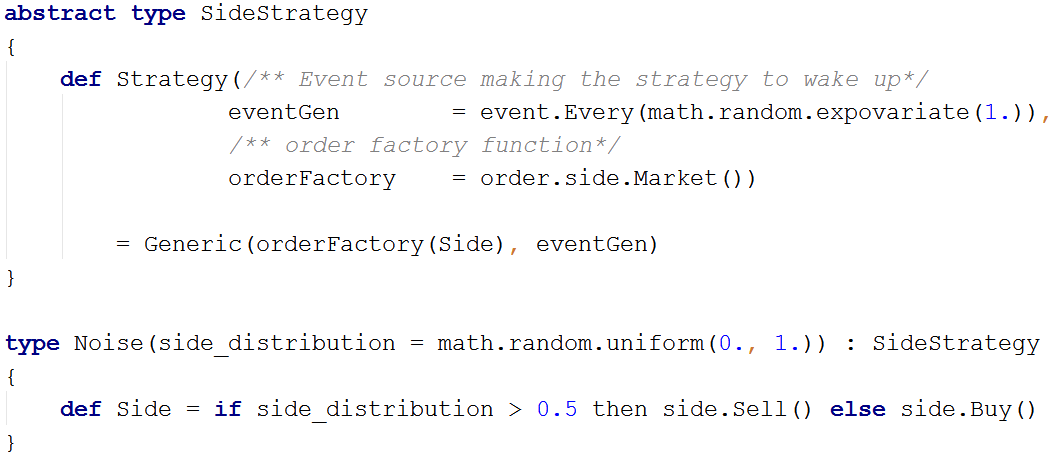
\includegraphics[width=1\linewidth]{side_strategy.png}
\end{frame}
%------------------------------------------------
\begin{frame}
\frametitle{Signal Strategy I}
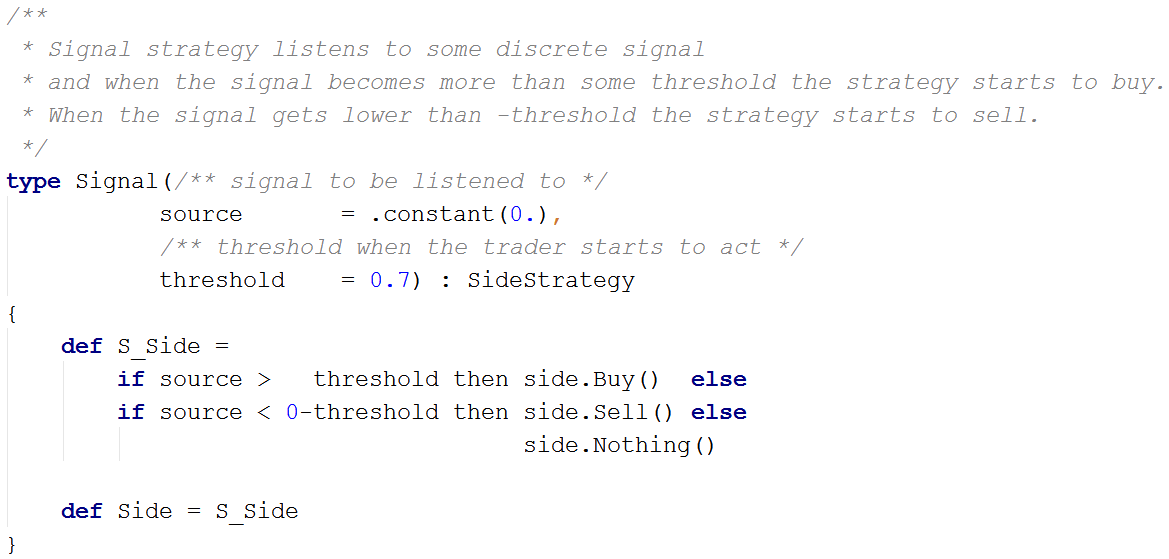
\includegraphics[width=1\linewidth]{signal_strategy.png}
\end{frame}
%------------------------------------------------
\begin{frame}
\frametitle{Signal Strategy II}
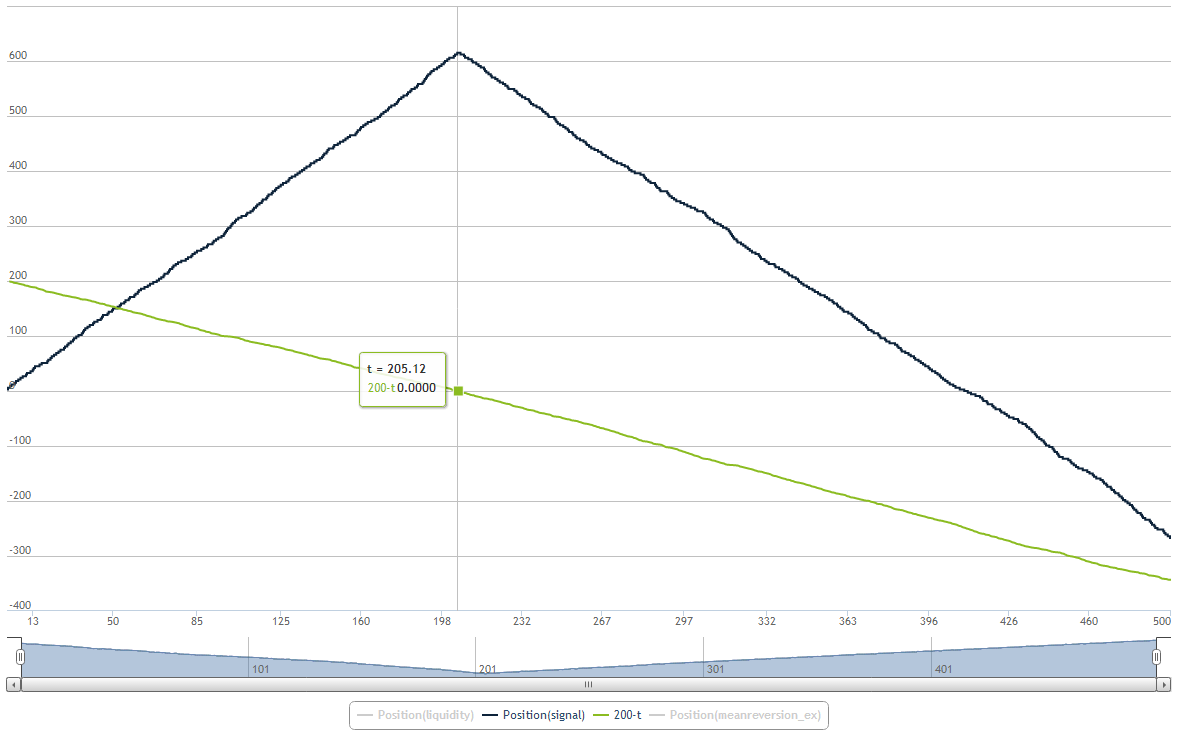
\includegraphics[width=1\linewidth]{signal.png}
\end{frame}
%------------------------------------------------
\begin{frame}
\frametitle{Trend Follower Strategy I}
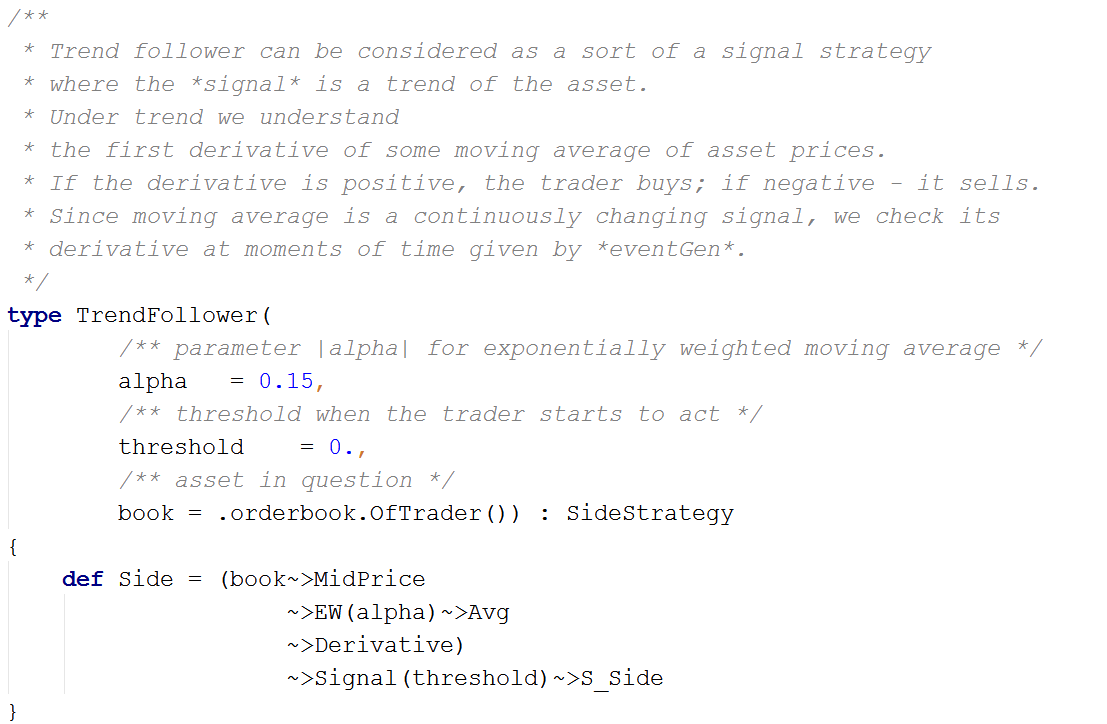
\includegraphics[width=1\linewidth]{trendfollower_strategy.png}
\end{frame}
%------------------------------------------------
\begin{frame}
\frametitle{Trend Follower Strategy II}
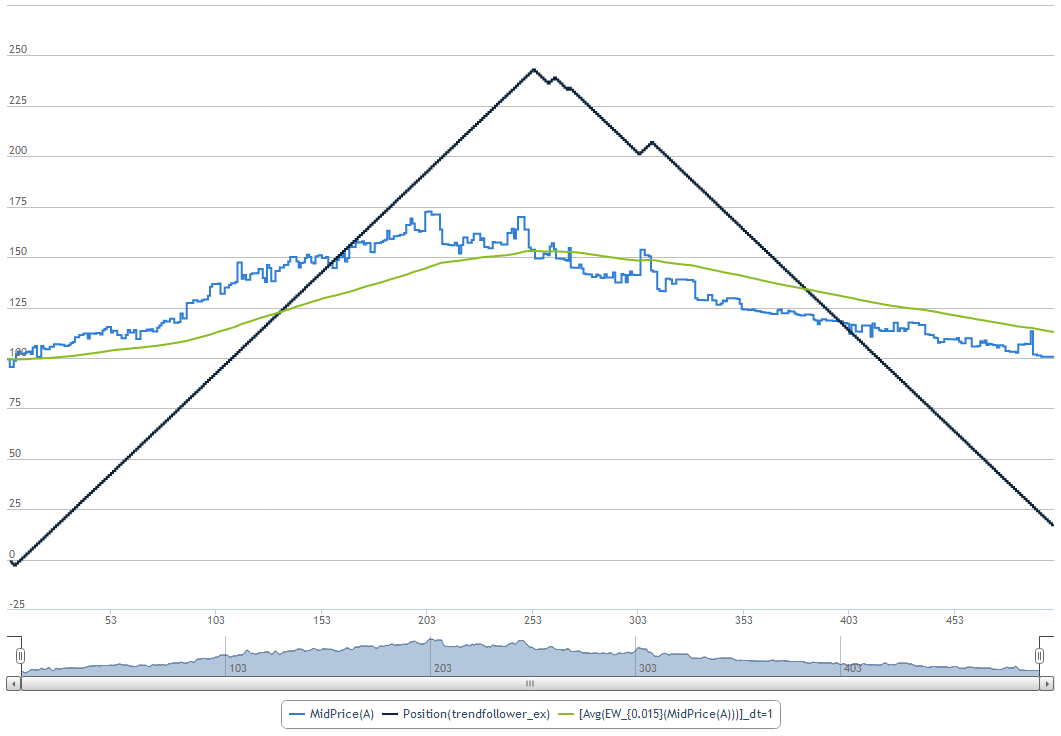
\includegraphics[width=1\linewidth]{trendfollower.png}
\end{frame}
%------------------------------------------------
\begin{frame}
\frametitle{Crossing Averages Strategy I}
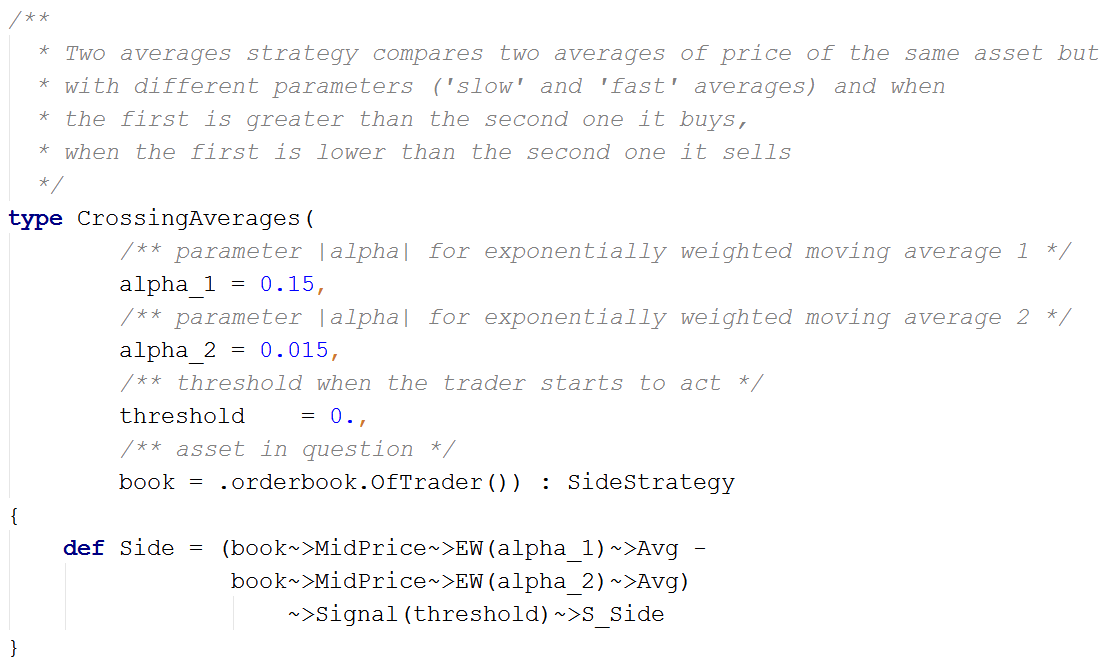
\includegraphics[width=1\linewidth]{twoaverages_strategy.png}
\end{frame}
%------------------------------------------------
\begin{frame}
\frametitle{Crossing Averages Strategy II}
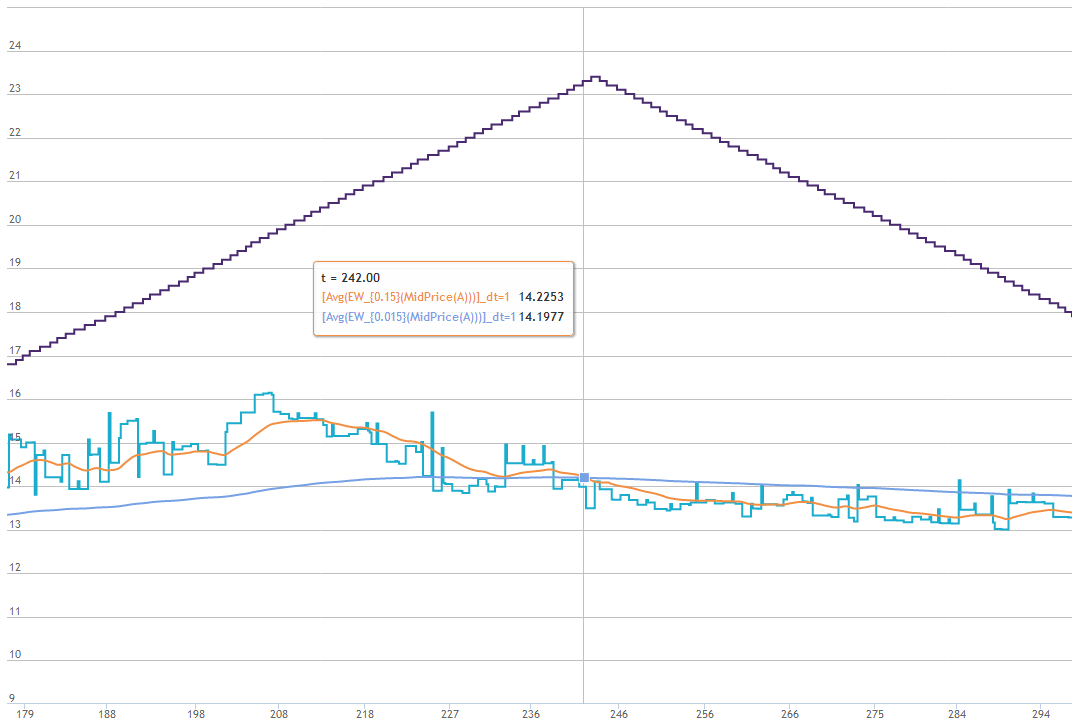
\includegraphics[width=1\linewidth]{twoaverages.png}
\end{frame}
%------------------------------------------------
\begin{frame}
\frametitle{Fundamental Value Strategy I}
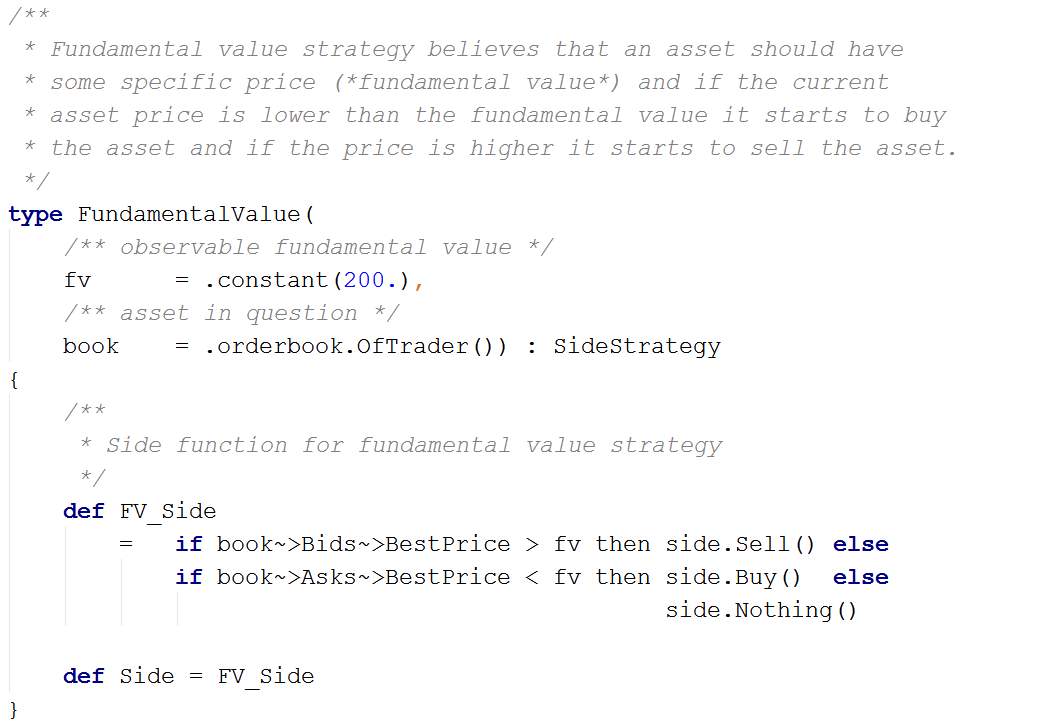
\includegraphics[width=1\linewidth]{fundamentalvalue_strategy.png}
\end{frame}
%------------------------------------------------
\begin{frame}
\frametitle{Fundamental Value Strategy II}
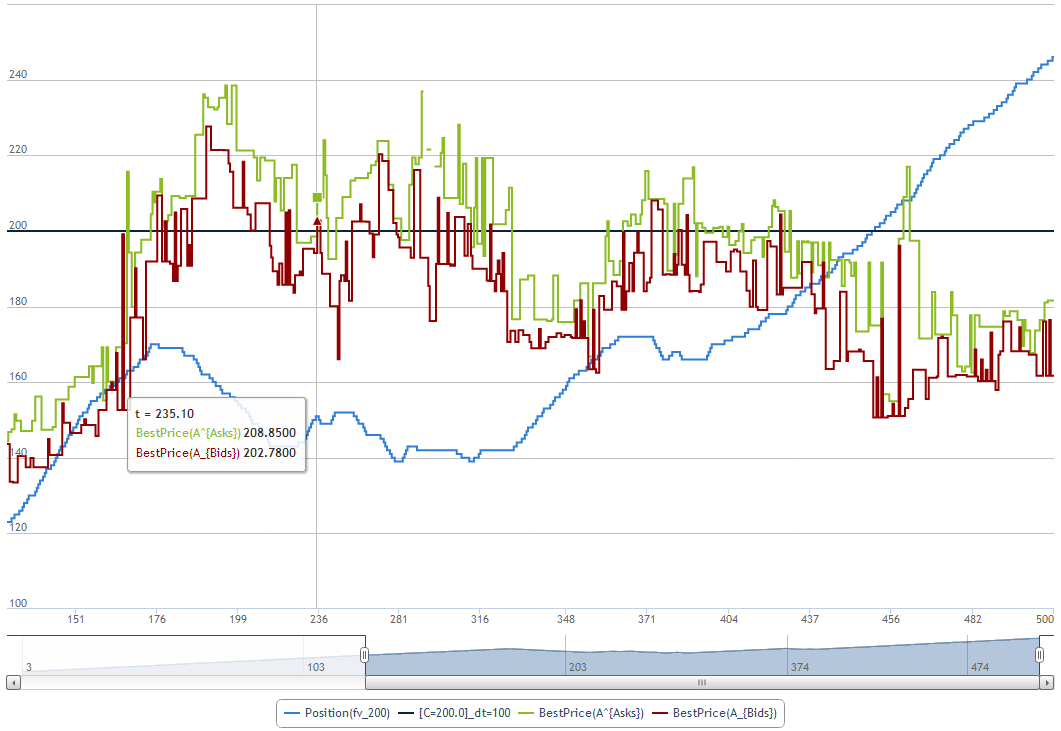
\includegraphics[width=1\linewidth]{fundamentalvalue.png}
\end{frame}
%------------------------------------------------
\begin{frame}
\frametitle{Mean Reversion Strategy I}
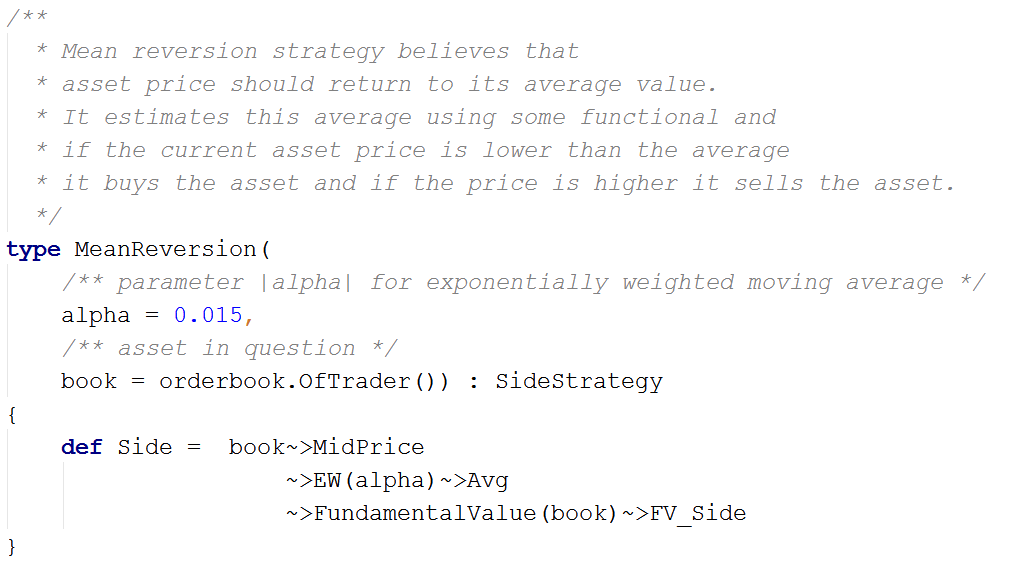
\includegraphics[width=1\linewidth]{meanreversion_strategy.png}
\end{frame}
%------------------------------------------------
\begin{frame}
\frametitle{Mean Reversion Strategy II}
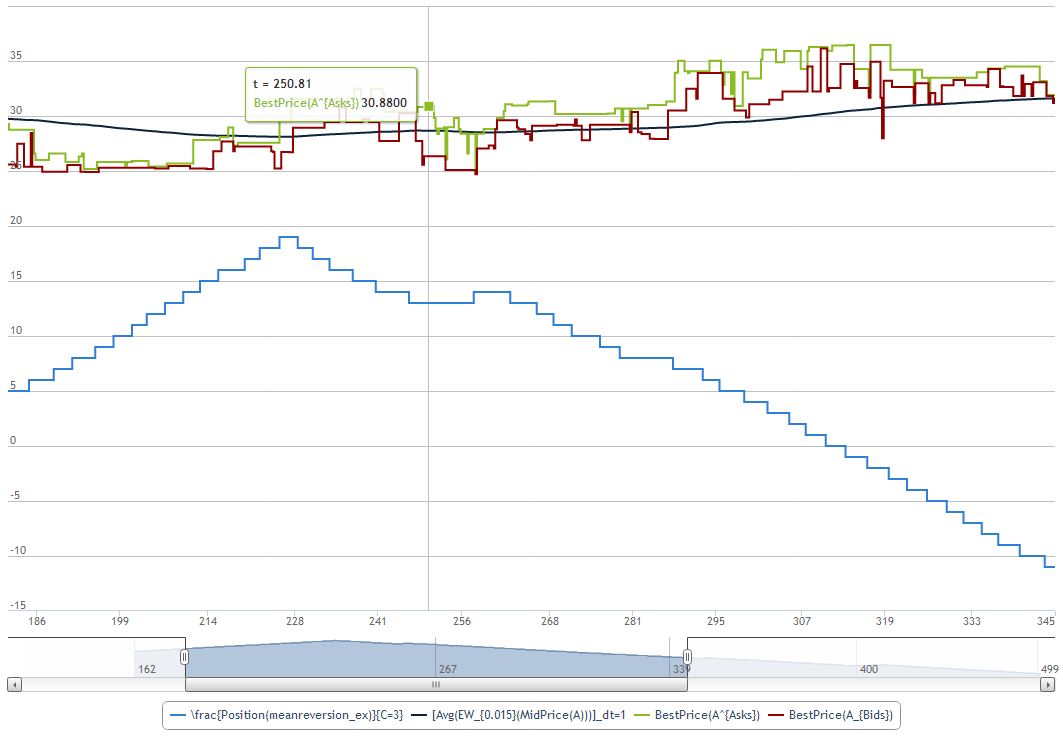
\includegraphics[width=1\linewidth]{meanreversion.png}
\end{frame}
%------------------------------------------------
\begin{frame}
\frametitle{Pair Trading Strategy I}
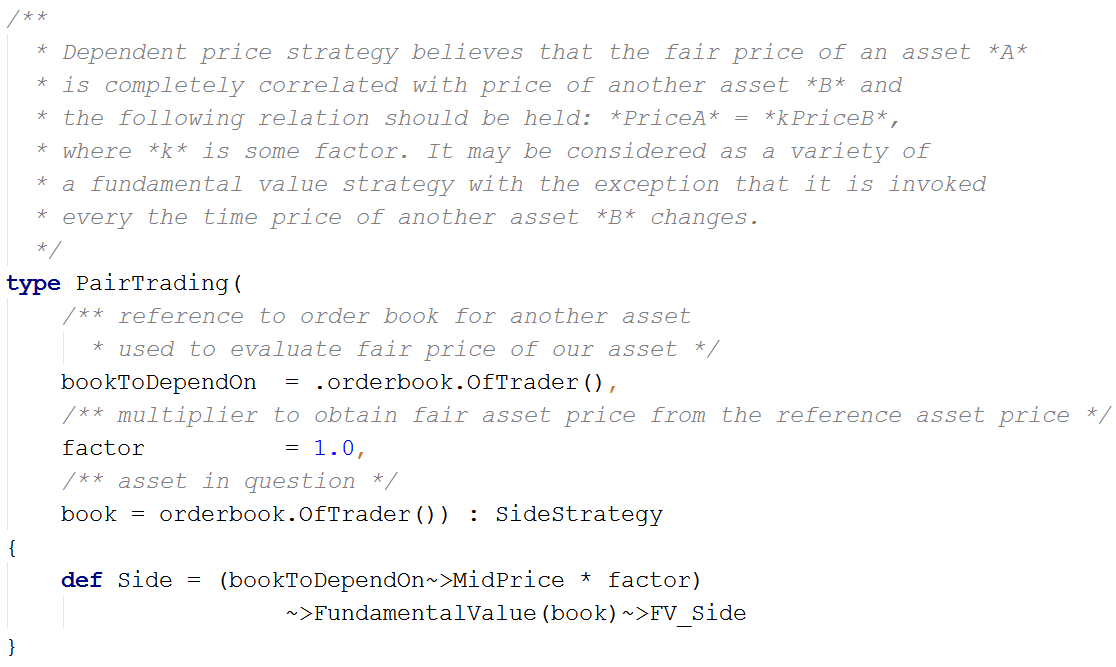
\includegraphics[width=1\linewidth]{dependency_strategy.png}
\end{frame}
%------------------------------------------------
\begin{frame}
\frametitle{Pair Trading Strategy II}
\includegraphics[width=1\linewidth]{dependency.png}
\end{frame}
%------------------------------------------------
\subsection{Price strategies}
\begin{frame}
\frametitle{Liquidity Provider Strategy}
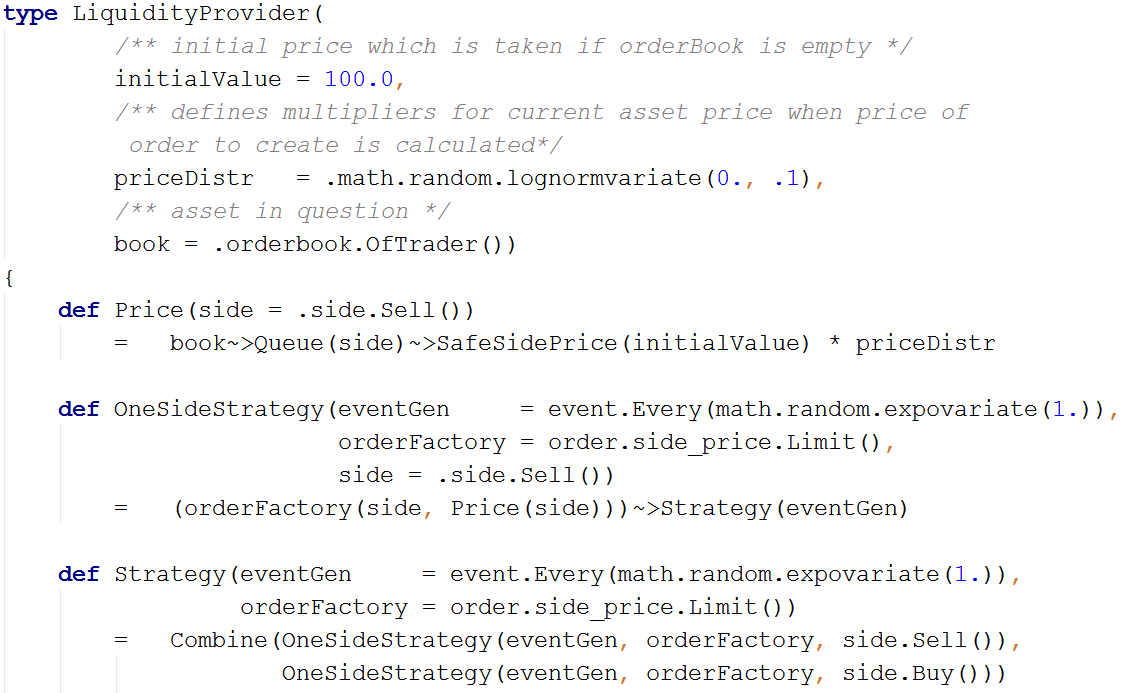
\includegraphics[width=1\linewidth]{lp_strategy.png}
\end{frame}
%------------------------------------------------
\begin{frame}
\frametitle{Market Data Strategy I}
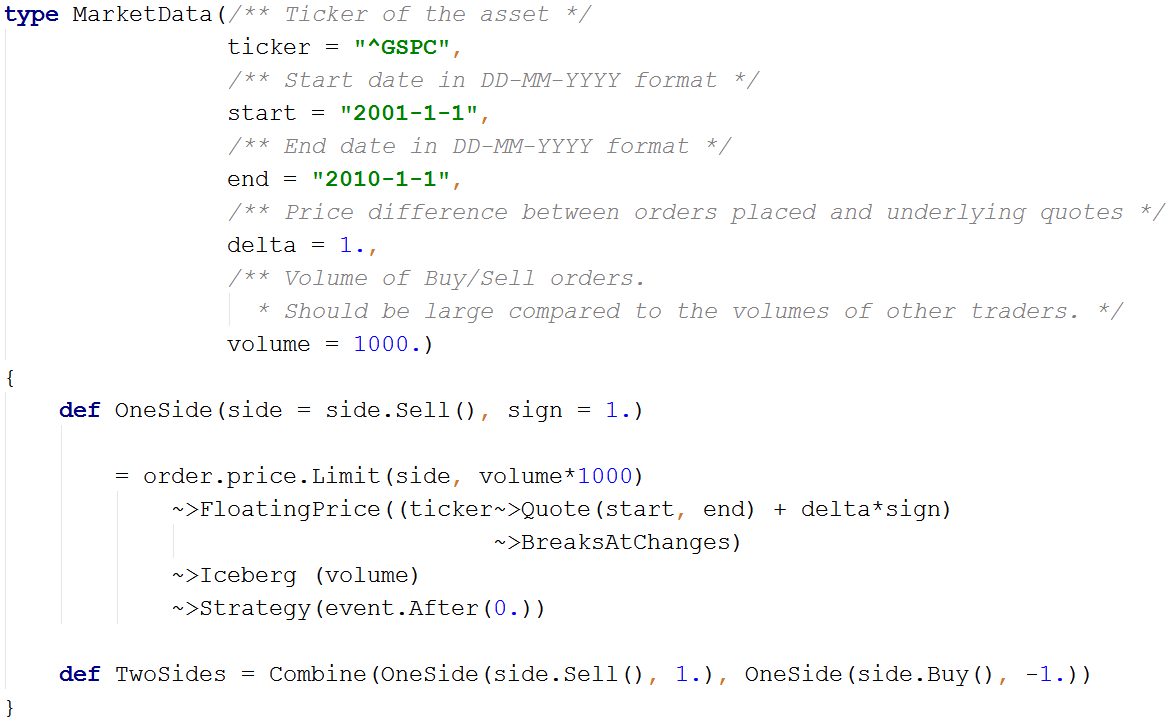
\includegraphics[width=1\linewidth]{marketdata_strategy.png}
\end{frame}
%------------------------------------------------
\begin{frame}
\frametitle{Market Data Strategy II}
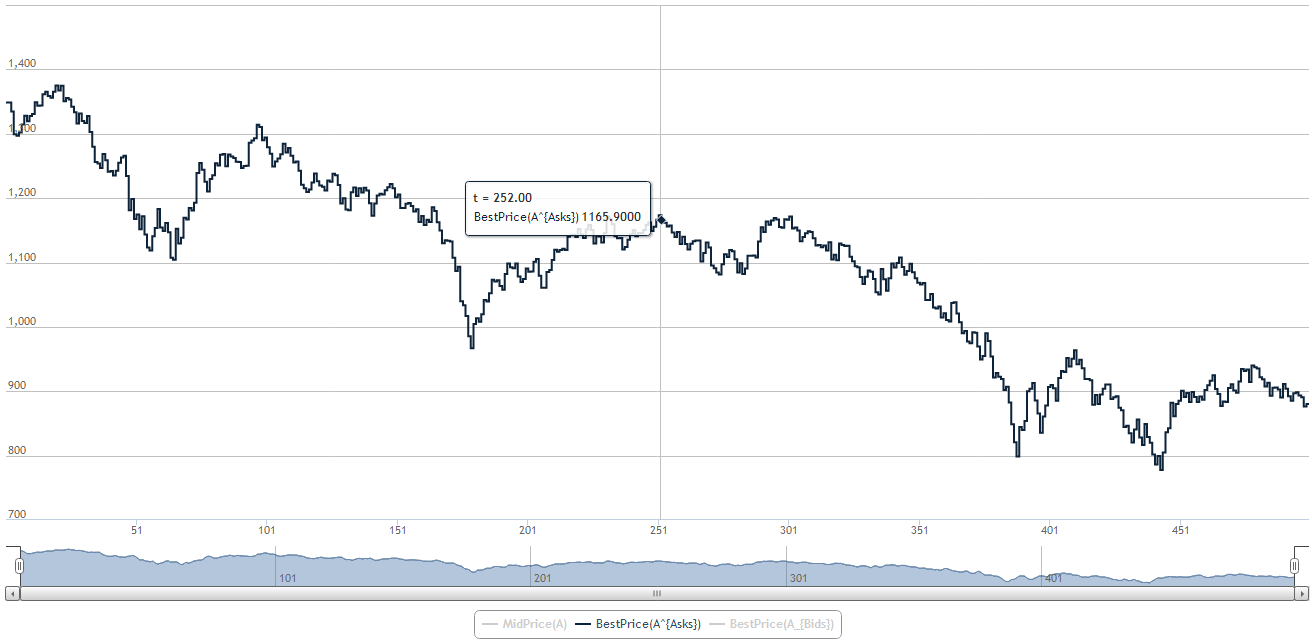
\includegraphics[width=1\linewidth]{marketdata.png}
\end{frame}
%------------------------------------------------
\begin{frame}
\frametitle{Market Maker Strategy I}
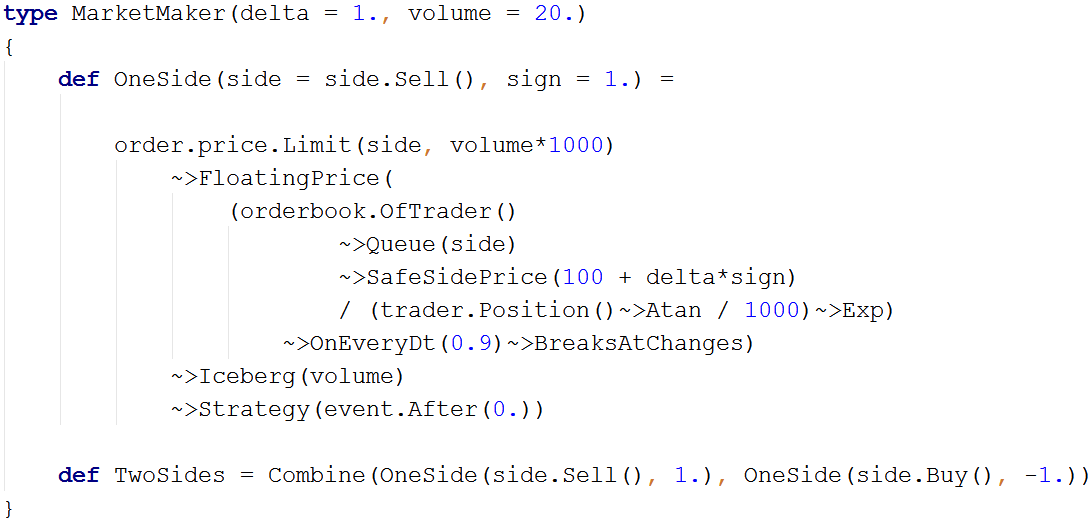
\includegraphics[width=1\linewidth]{marketmaker_strategy.png}
\end{frame}
%------------------------------------------------
\begin{frame}
\frametitle{Market Maker Strategy II}
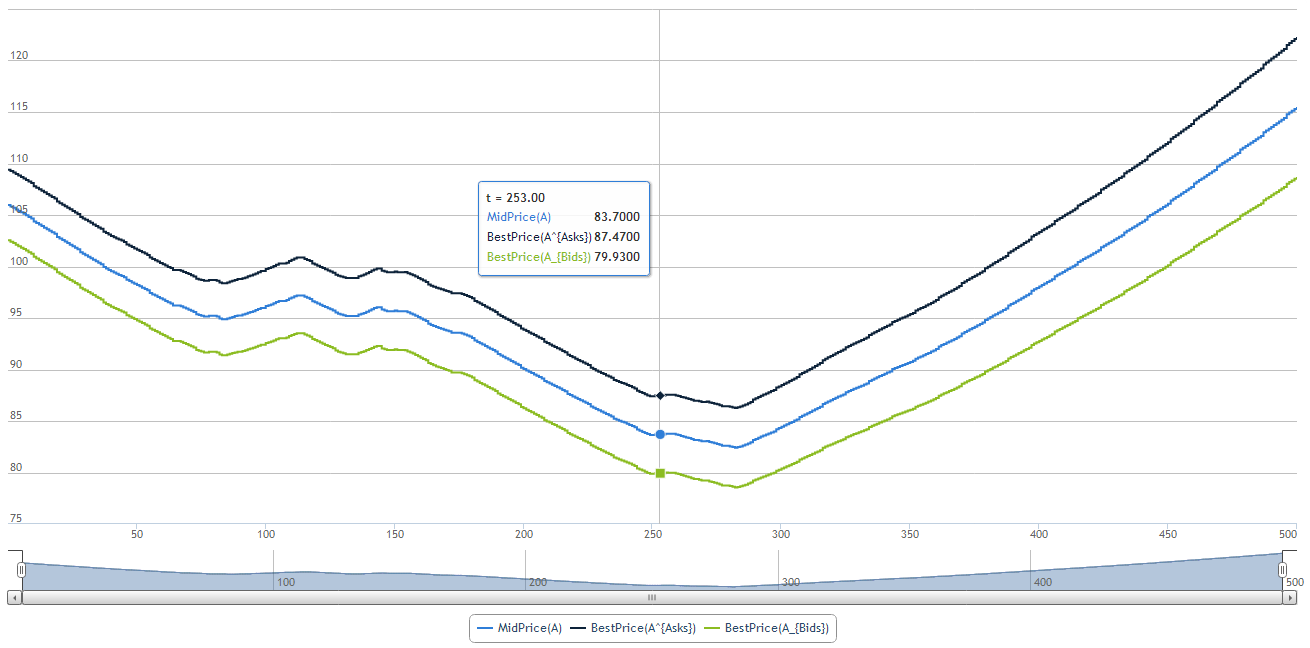
\includegraphics[width=1\linewidth]{marketmaker.png}
\end{frame}
%------------------------------------------------
\subsection{Adaptive strategies}
\begin{frame}
\frametitle{Trade-If-Profitable Strategy I}
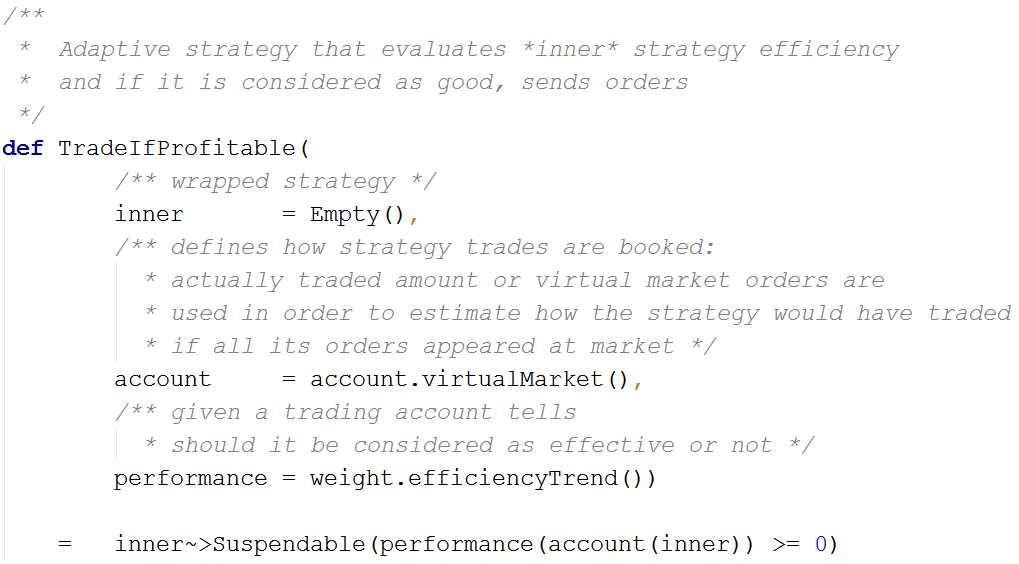
\includegraphics[width=1\linewidth]{tradeifprofitable_strategy.png}
\end{frame}
%------------------------------------------------
\begin{frame}
\frametitle{Trade-If-Profitable Strategy II}
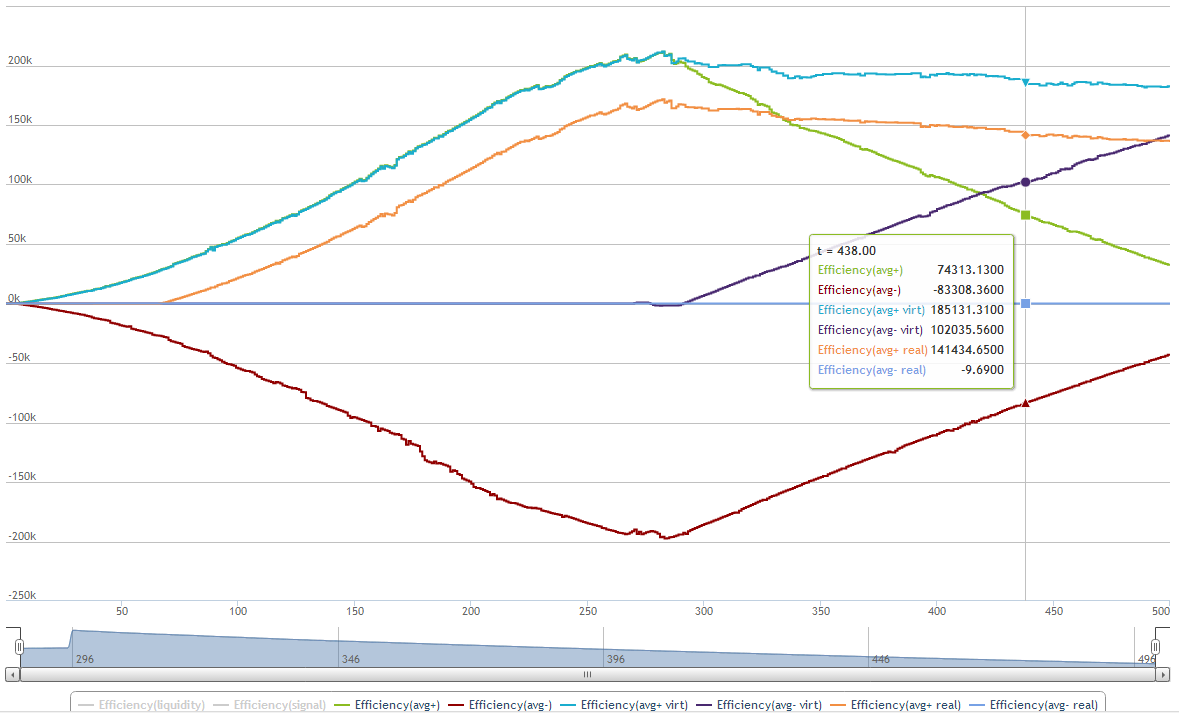
\includegraphics[width=1\linewidth]{tradeifprofitable.png}
\end{frame}
%------------------------------------------------
\begin{frame}
\frametitle{Choose-the-best strategy}
Backtests aggregated strategies and allows to run only to that one who has the best performance. By default, first derivative of a moving average of 'cleared' trader's balance is used to evaluate the efficiency.
\begin{figure}[htbp]
\centering
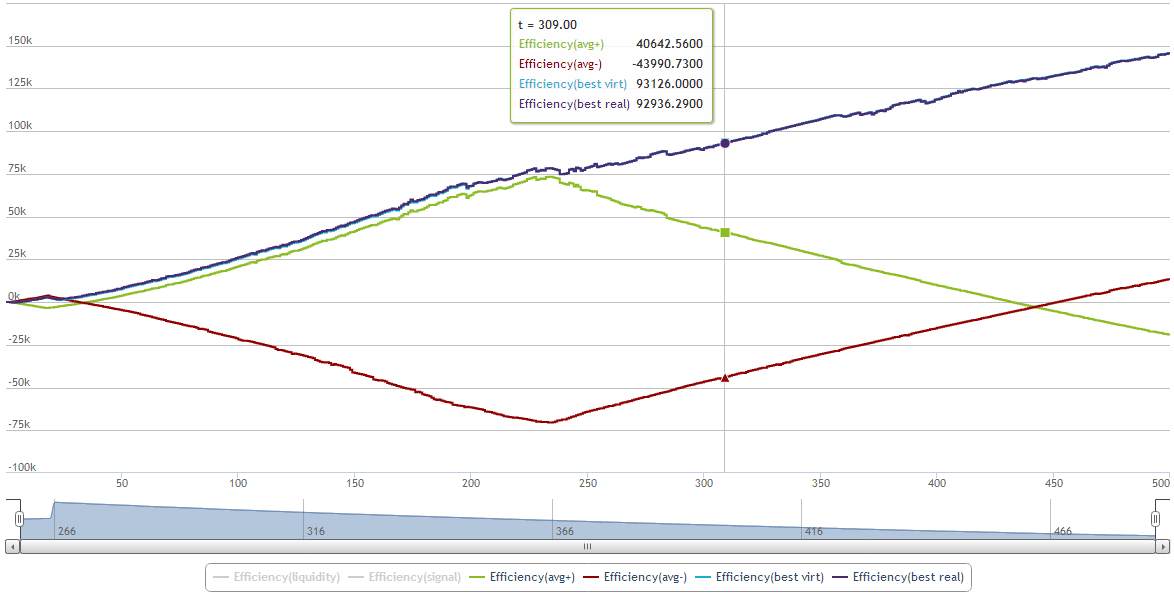
\includegraphics[width=1\linewidth]{choosethebest.png}
\end{figure}
\end{frame}
%------------------------------------------------
\begin{frame}
\frametitle{Multiarmed Bandit Strategy I}
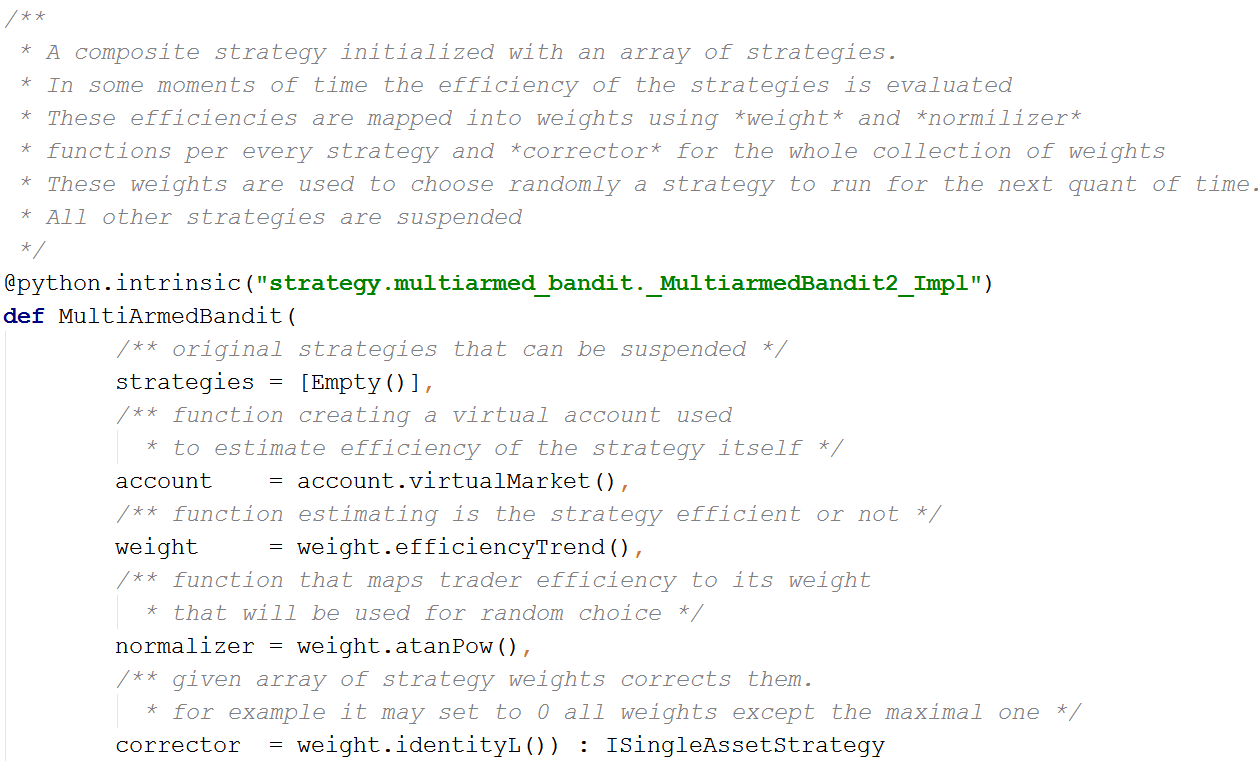
\includegraphics[width=1\linewidth]{multiarmedbandit_strategy.png}
\end{frame}
%------------------------------------------------
\begin{frame}
\frametitle{Multiarmed Bandit Strategy II}
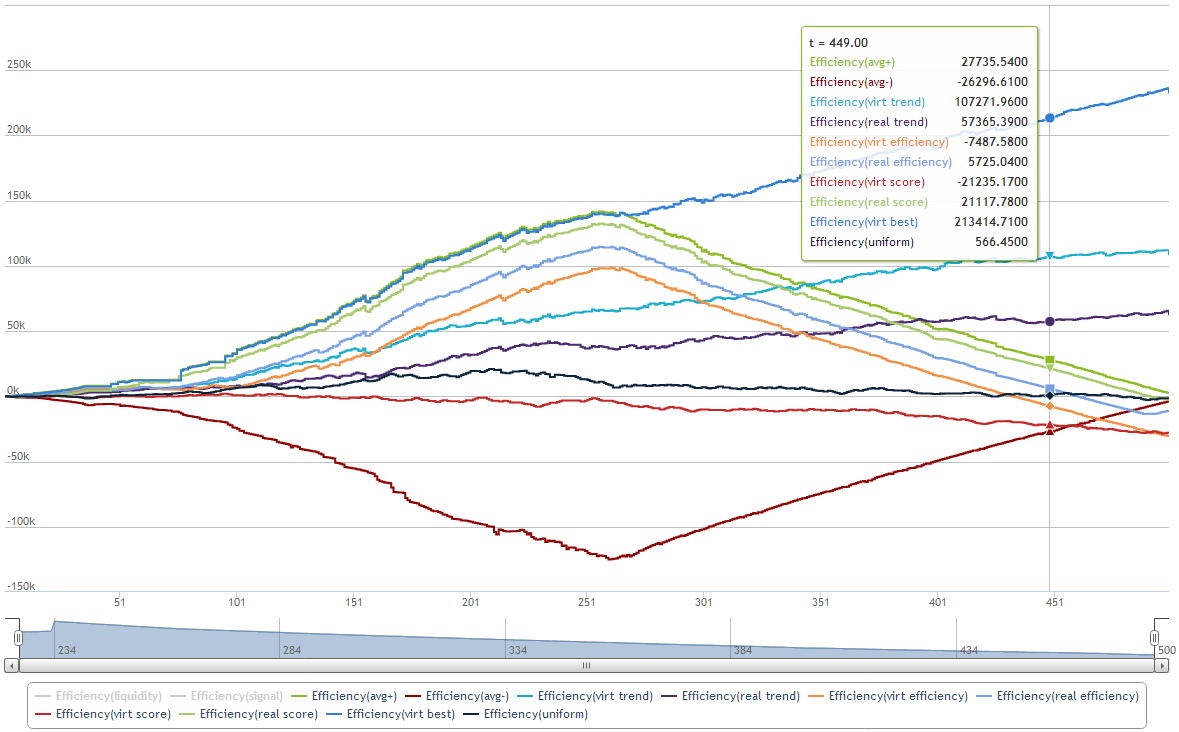
\includegraphics[width=1\linewidth]{multiarmedbandit.png}
\end{frame}
%------------------------------------------------
\begin{frame}
\frametitle{Arbitrage Strategy}
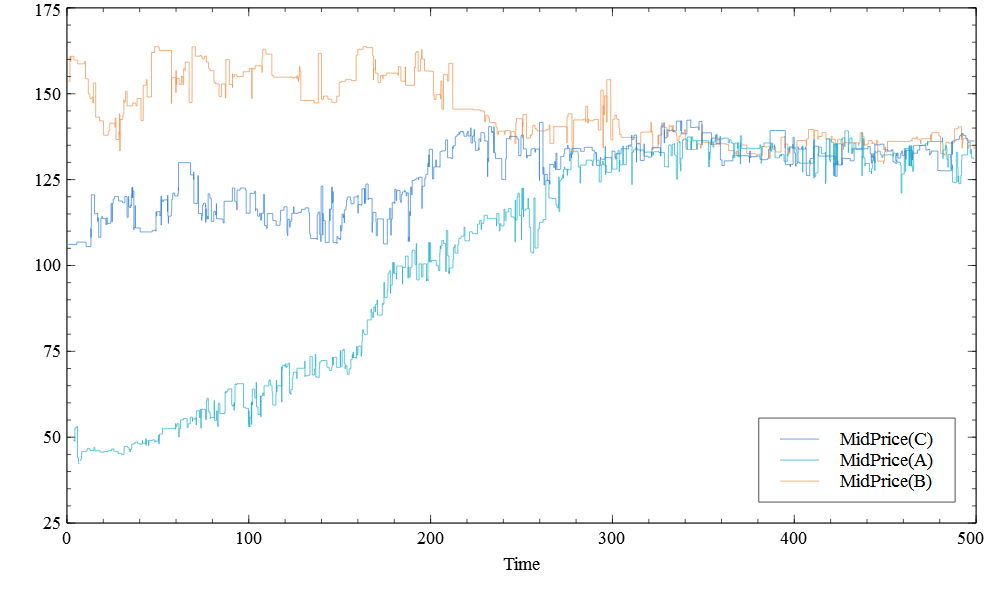
\includegraphics[width=1\linewidth]{Arbitrage.png}
\end{frame}
%------------------------------------------------

\section{Simulator components}

\begin{frame}
\frametitle{Simulator components}
\begin{figure}[htbp]
\centering
\includegraphics[width=1\linewidth]{objects.png}
\end{figure}
\end{frame}

\begin{frame}
\frametitle{Scheduler}
\begin{itemize}
  \item Main class for every discrete event simulation system.
  \item Maintains a set of actions to fulfill in future and launches them according their action times: from older ones to newer.
\end{itemize}
Interface:
\begin{itemize}
  \item Event scheduling:
  \begin{itemize}
    \item \texttt{schedule(actionTime, handler)}
    \item \texttt{scheduleAfter(dt, handler)}
  \end{itemize}
  \item Simulation control:
  \begin{itemize}
    \item \texttt{workTill(limitTime)}
    \item \texttt{advance(dt)}
    \item \texttt{reset()}
  \end{itemize}
\end{itemize}
\end{frame}

\begin{frame}
\frametitle{Events}
\begin{itemize}
  \item \texttt{event.Event}. Base class for multicast events.
  \item \texttt{event.Conditional}. Multicast event class with conditional events support. Allows effective notification mechanism for collections of event handler of form \texttt{event.GreaterThan(x, listener)} and \texttt{event.LessThan(x, listener)}. Internally it keeps two dequeues of event handlers sorted by their trigger values and notifies only those handlers whose trigger conditions are fullfilled.
  \item \texttt{event.GreaterThan(x, listener)}. Fires \texttt{listener} only if the value observed is greater than \texttt{x}.
  \item \texttt{event.LessThan(x, listener)}. Fires \texttt{listener} only if the value observed is less than \texttt{x}.
\end{itemize}
\end{frame}

%------------------------------------------------
\begin{frame}
\frametitle{Order book}
\begin{itemize}
  \item Represents a single asset traded in some market (Same asset traded in different markets would be represented by different order books)
  \item Matches incoming orders
  \item Stores unfulfilled limit orders in two order queues (\texttt{Asks} for sell orders and \texttt{Bids} for buy orders)
  \item Corrects limit order price with respect to tick size
  \item Imposes order processing fee
  \item Supports queries about order book structure
  \item Notifies listeners about trades and price changes
\end{itemize}
\end{frame}

%------------------------------------------------
\begin{frame}
\frametitle{Order book for a remote trader}
\begin{itemize}
  \item Models a trader connected to a market by a communication channel with non-negligible latency
  \item Introduces delay in information propagation from a trader to an order book and vice versa (so a trader has outdated information about market and orders are sent to the market with a certain delay)
  \item Assures correct order of messages: older messages always come earlier than newer ones
\end{itemize}
\end{frame}

%------------------------------------------------
\begin{frame}
\frametitle{Basic orders}
Orders supported internally by an order book:
\begin{itemize}
  \item \texttt{Market(side, volume)}
  \item \texttt{Limit(side, price, volume)}
  \item \texttt{Cancel(limitOrder)}
\end{itemize}
Limit and market orders notifies their listeners about all trades they take part in.
Factory functions are usually used in order to create orders.
\end{frame}

%------------------------------------------------
\begin{frame}
\frametitle{Meta orders I}
Follow order interface from trader's perspective (so they can be used instead of basic orders) but behave like a sequence of base orders from an order book point of view.
\begin{itemize}
  \item \texttt{Iceberg(volumeLimit, underlyingFactory)} splits orders created by \texttt{underlyingFactory} to pieces with volume less than \texttt{volumeLimit} and sends them one by one to an order book ensuring that only one order at time is processed there
  \item \texttt{FloatingPrice(price, underlyingFactory)} listens to an observable \texttt{price} and when it changes, cancels its order on the markets and resends it with the new price.  
  \item \texttt{Peg(underlyingFactory)} creates a limit-like order with given volume and the most attractive price, sends it to an order book and if the order book best price changes, cancels it and resends with a better price. Implemented via \texttt{FloatingPrice}.
\end{itemize}
\end{frame}

%------------------------------------------------
\begin{frame}
\frametitle{Meta orders II}
\begin{itemize}
  \item \texttt{WithExpiry(lifetime, underlyingFactory)} sends a limit-like order and after \texttt{lifetime} cancels it
  \item \texttt{ImmediateOrCancel(underlyingFactory)} is like \texttt{WithExpiry} but with \texttt{lifetime} equal to 0 making a limit order to act as a conditional market order
  \item \texttt{StopLoss(lossFactor, underlyingFactory)} order is initialised by an underlying order and a maximal acceptable loss factor.
      It keeps track of position and balance change induced by trades of the underlying order and
      if losses from keeping the position exceed certain limit (given by maximum \texttt{lossFactor}),
      the meta order clears its position.
\end{itemize}
\end{frame}

%------------------------------------------------
\begin{frame}
\frametitle{Traders}
Single asset traders
\begin{itemize}
  \item send orders to order books
  \item bookkeep their position and balance
  \item run a number of trading strategies
  \item notify listeners about trades done and orders sent
\end{itemize}
Single asset traders operate on a single or multiple markets.
Multiple asset traders are about to be added.
\end{frame}
%------------------------------------------------
\begin{frame}
\frametitle{Observable}
Traders and order books provide basic accessors to their current state but don't collect any statistics. In order to do it in an interoperable way a notion of observable value was introduced: it allows to read its current value and notifies listeners about its change. Examples of observables are:
\begin{itemize}
    \item on traders: position, balance, market value of the portfolio, 'cleared' balance etc.
    \item on order books: ask/mid/bid price, last trade price, price at volume, volume of orders with price better than given one etc.
    \item \texttt{OnEveryDt(dt, dataSource)} evaluates \texttt{dataSource} every \texttt{dt} moments of time.
\end{itemize}
History of an observable can be stored in a \texttt{TimeSerie} and rendered later on a graph.
\end{frame}
%------------------------------------------------

\section{GUIs: Veusz and Web}
\begin{frame}
\frametitle{Using Veusz}
When developing a new strategy it is reasonable to test it using scripts and visualize results by Veusz
\begin{figure}[htbp]
\centering
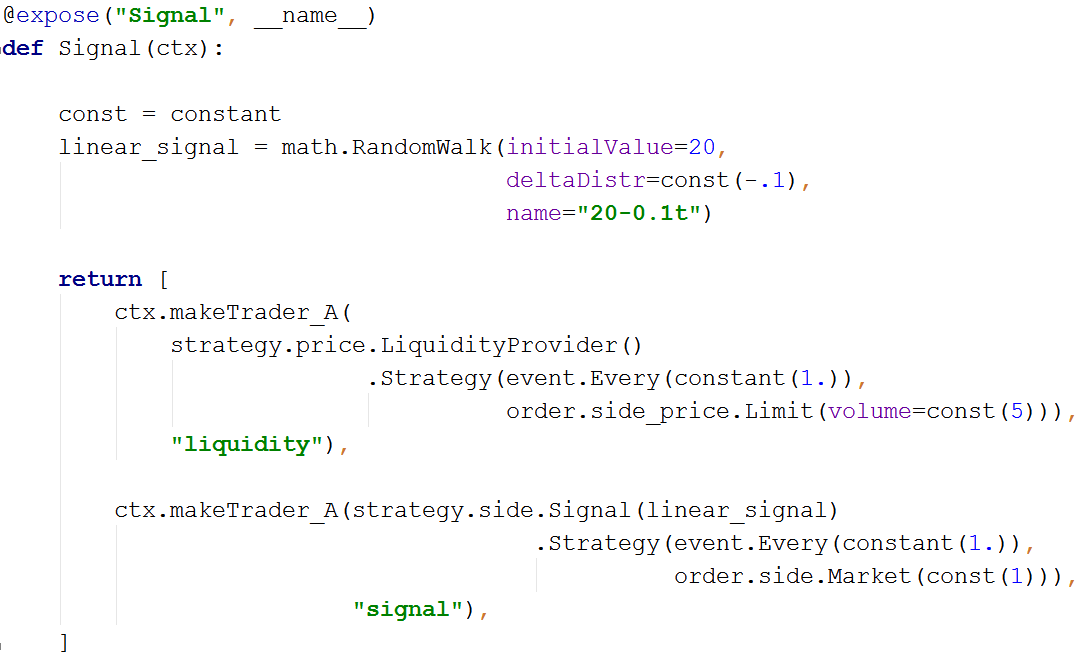
\includegraphics[width=1\linewidth]{using_veusz_code.png}
\end{figure}
\end{frame}

%------------------------------------------------
\begin{frame}
\frametitle{Rendering graphs by Veusz}
\begin{figure}[htbp]
\centering
\includegraphics[width=1\linewidth]{veusz_graph.png}
\end{figure}
\end{frame}

%------------------------------------------------

\begin{frame}
\frametitle{Web interface}
Web interface allows to compose a market to simulate from existing objects and set up their parameters
\begin{figure}[htbp]
\centering
\includegraphics[width=1\linewidth]{js-help.png}
\end{figure}
\end{frame}

\begin{frame}
\frametitle{Time series}
Timeseries field of a trader or an order book instructs what data should be collected and rendered on graphs
\begin{figure}[htbp]
\centering
\includegraphics[width=1\linewidth]{js-timeserie.png}
\end{figure}
\end{frame}

\begin{frame}
\frametitle{Rendering results}
\begin{figure}[htbp]
\centering
\includegraphics[width=1\linewidth]{js-graph.png}
\end{figure}
\end{frame}

\begin{frame}
\frametitle{Node aliases}
\begin{figure}[htbp]
Object tree nodes can be assigned aliases that can be used later to refer to the sub-tree (explicit by-value or by-reference cloning semantics is to be implemented)
\centering
\includegraphics[width=1\linewidth]{js-alias.png}
\end{figure}
\end{frame}

\begin{frame}
\frametitle{Workspaces}
\begin{figure}[htbp]
Every user (identified by browser cookies) may switch between multiple workspaces. Workspaces can be forked, removed or created from a set of predefined ones.
\centering
\includegraphics[width=1\linewidth]{js-fork.png}
\end{figure}
\end{frame}

\begin{frame}
\frametitle{Installation}
\begin{itemize}
\item OS supported: Linux, Mac OS X, Windows
\item Browsers supported: Chrome, Firefox, Safari, Opera
\item Scala 10.2 can be installed using \textcolor[rgb]{0.00,0.50,0.75}{\href{http://www.scala-sbt.org/release/docs/Getting-Started/Setup.html}{SBT}}
\item Python 2.7  
\item Python packages can be installed using \texttt{pip} or \texttt{easyinstall}:
\begin{itemize}
\item \textcolor[rgb]{0.00,0.50,0.75}{\href{http://home.gna.org/veusz/}{Veusz}} (for graph plotting)
\item \textcolor[rgb]{0.00,0.50,0.75}{\href{http://flask.pocoo.org}{Flask}} and \textcolor[rgb]{0.00,0.50,0.75}{\href{https://pypi.python.org/pypi/docutils}{Docutils}} (to run a Web-server)
\item \textcolor[rgb]{0.00,0.50,0.75}{\href{https://pypi.python.org/pypi/blist/}{Blist}} (sorted collections used by ArbitrageTrader)
\item \textcolor[rgb]{0.00,0.50,0.75}{\href{http://pandas.pydata.org/}{Pandas}} (only needed for \texttt{observable.Quotes} at the moment)
\item \textcolor[rgb]{0.00,0.50,0.75}{\href{https://pypi.python.org/pypi/numpy}{Numpy}} (only needed for \texttt{strategy.MultiArmedBandit} at the moment)
\end{itemize}
\item Source code downloadable from \textcolor[rgb]{0.00,0.50,0.75}{\href{https://github.com/fiquant/marketsimulator}{GitHub}}
\item Latest public version of the simulator can be downloaded from \textcolor[rgb]{0.00,0.50,0.75}{\href{https://github.com/fiquant/marketsimulator/releases}{here}}.
\item Online documentation can be found \textcolor[rgb]{0.00,0.50,0.75}{\href{https://github.com/fiquant/marketsimulator/blob/master/README.rst}{here}}.
\end{itemize}

\end{frame}

\begin{frame}
\Huge{\centerline{Thank you!}}
\end{frame}

%----------------------------------------------------------------------------------------

\end{document} 